\documentclass[tikz,border=8pt]{standalone}
% Shared look for every TikZ diagram. Load with \input{../../tools/tikz-style.tex}
\usepackage[T1]{fontenc}
\usepackage{lmodern}
\renewcommand{\sfdefault}{lmr}  % diagrams use the same serif as the text
\usetikzlibrary{arrows.meta, positioning, shapes.geometric, calc, fit, backgrounds}
\definecolor{cblue}{HTML}{4C78A8}
\definecolor{corange}{HTML}{F58518}
\definecolor{cgreen}{HTML}{54A24B}
\definecolor{cred}{HTML}{E45756}
\definecolor{cpurple}{HTML}{B279A2}
\definecolor{cgrey}{HTML}{6B6B6B}
\tikzset{
  every picture/.style={font=\sffamily, line width=1.2pt},
  box/.style={draw=#1, fill=#1!12, rounded corners=4pt, align=center, inner sep=7pt, minimum height=1.1cm},
  box/.default=cgrey,
  arrow/.style={-{Stealth[length=3mm]}, draw=cgrey, line width=1.4pt},
  title/.style={font=\sffamily\bfseries\Large},
  note/.style={font=\sffamily\small, text=cgrey, align=center},
}
\AtBeginDocument{\hyphenpenalty=10000 \exhyphenpenalty=10000}

\begin{document}
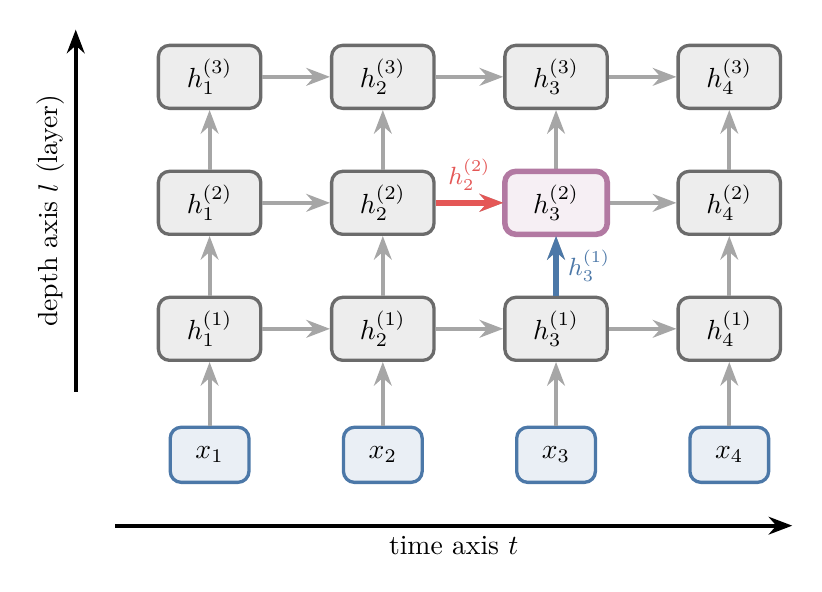
\begin{tikzpicture}[cell/.style={box=#1, minimum width=1.3cm, minimum height=0.8cm, inner sep=2pt}]
  \foreach \l in {1,2,3} \foreach \t in {1,2,3,4} {
    \node[cell=cgrey] (c\t\l) at (2.2*\t, 1.6*\l) {$h^{(\l)}_\t$};
  }
  \foreach \t in {1,2,3,4} {
    \node[box=cblue, minimum width=1.0cm, minimum height=0.7cm, inner sep=2pt] (x\t) at (2.2*\t,0) {$x_\t$};
    \draw[arrow, draw=cgrey!60] (x\t) -- (c\t1);
    \draw[arrow, draw=cgrey!60] (c\t1) -- (c\t2);
    \draw[arrow, draw=cgrey!60] (c\t2) -- (c\t3);
  }
  \foreach \l in {1,2,3} {
    \draw[arrow, draw=cgrey!60] (c1\l) -- (c2\l);
    \draw[arrow, draw=cgrey!60] (c2\l) -- (c3\l);
    \draw[arrow, draw=cgrey!60] (c3\l) -- (c4\l);
  }
  % highlighted cell: t = 3, layer 2
  \node[cell=cpurple, line width=2pt] at (c32) {$h^{(2)}_3$};
  \draw[arrow, draw=cred, line width=2pt] (c22) -- node[above, note, text=cred] {$h^{(2)}_{2}$} (c32);
  \draw[arrow, draw=cblue, line width=2pt] (c31) -- node[right, note, text=cblue] {$h^{(1)}_{3}$} (c32);
  % axes
  \draw[arrow, draw=black] (1.0,-0.9) -- node[below] {time axis $t$} (9.6,-0.9);
  \draw[arrow, draw=black] (0.5,0.8) -- node[above, rotate=90] {depth axis $l$ (layer)} (0.5,5.4);
\end{tikzpicture}
\end{document}
